\section{Thickness and size of the shield}
The thickness and size of the shield can be estimated by considering a real material. The shield material should have a large electric conductivity $\sigma$ and should therefore behave like an conductor. Even a superconducting shield could be considered.
For a real metal like for example copper, the transmission $T$ of electromagnetic waves is given by \cite{Vandenbosch_2022}
\begin{equation}
  T = \abs{\frac{\vec{E}_\mathrm{after}}{\vec{E}_\mathrm{before}}} = \frac{2}{Z_0 \sigma d}
\end{equation}
where $\sigma$ is the electric conductivity, $Z_0 = 377\si{\Omega}$ the impedance of free space (provided the shield is placed in a vacuum or air) and $d$ the thickness of the shield.
The electric conductivity has a strong dependence on temperature and decreases with $1/T^5$ \footnote{This behavior is only true for temperatures below the Debye temperature. For copper, this limit is around $\Theta_D = 343\si{K}$. In the experiment, the shield is cooled down, so the low-temperature limit of the electric conductivity for metals is very valid \cite{Berman_1952}.} with increasing temperatures \cite[p. 284-286]{Gross_2018}. The electric conductivity for copper at room temperature ($\sigma = 59.6\times 10^6 \si{S/m}$) should therefore be a very valid worst-case approximation. 
Measured data suggest a conductivity of $\sigma(T = 10) \approx 1.5\times 10^{10}\si{S/m}$ \cite{Berman_1952}.

To estimate the thickness of the shield, I am using the condition, that entanglement between the masses should be built up mainly due to gravity. All other possible interactions like Coulomb or Casimir forces, should be suppressed by the shield.
To quantify the amount of entanglement built-up over time, I obt for a measure I call \emph{entanglement rate}.
This rate $\Gamma$ can be calculated like
\begin{equation}\label{eq:4:entanglement-rate}
  \Gamma = \pdv{t} E_N(\rho)\Big|_{t=0}
\end{equation} 
where $E_N$ is an appropriate entanglement measure - in this case the logarithmic negativity from \cref{sec:2:entanglement-measures}.
For the gravitational entanglement, this can be calculated by eq. \eqref{eq:2:entanglement-dynamics-parallel} and for the parallel configuration this is given by
\begin{equation}\label{eq:4:entanglement-rate-gravity}
  \Gamma_\mathrm{Gravity} = \frac{G M_A M_B (\Delta x)^2}{16 \hbar L^3 \log 2} .
\end{equation}
The entanglement rate for other interactions should be smaller (and ideally a lot smaller) than the entanglement rate due to gravity.
In the following, this is considered for Coulomb- and Casimir interactions.

\subsection{Shielding Coulomb-Interactions}
The main focus of the shield is to block electromagnetic interactions between the spheres. A very simple example is the Coulomb interaction which arises, if the masses cary a small amount of charge. 
The Coulomb interaction potential
\begin{equation}
  V = \frac{1}{4\pi\varepsilon}
\end{equation}

\begin{figure}[!htbp]
  \centering
  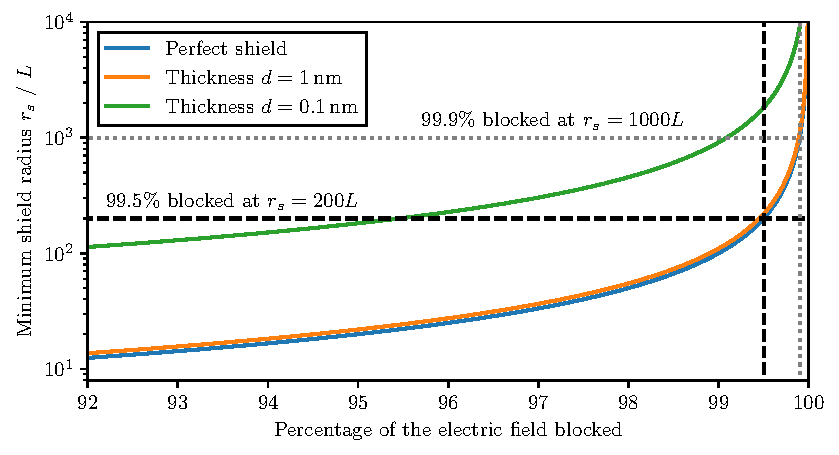
\includegraphics[width=\textwidth]{./../figures/shield-radius.pdf}
  \label{fig:4:shield-radius}
  \caption{Radius of the shield depending on the amount of the electromagnetic field blocked and for different thicknesses $d$. For a shielding between $99.5...99.9\%$, a radius of at least $r_s =200...1000L$ should be used. For a sphere-plate distance of $L=2 \times 10^{-5}\si{m}$, the shield radius should be in the order of millimeters and centimeters. The lines for selected thicknesses where computed at room temperature.}
\end{figure}



\subsection{Shielding Casimir-Interactions}



\subsection{Gravitational effects of the shield}
For simplicity, in the following estimations of the attractive gravitational force between an infinitely large plate with thickness $d$ and a sphere positioned a distance $L$ in front of the plate is calculated. This should slightly overestimate the actual force due to a finite plate \footnote{In fact, using a finite shield with radius $r_s = 0.01\si{m}$, the total force decreases only by $0.2\%$ compared to an infinitely sized one.}.
The gravitational force between the sphere and a infinitesimal mass segment $\dd m = r \rho d \dd r\dd \varphi$ of the plate with density $\rho$ at a distance $r$ from the center is given by
\begin{equation}
  \dd \vec{F} = \frac{G M \dd m}{\ell^2} \boldsymbol{\hat{\ell}} 
  \quad \Rightarrow \quad
  \dd F_z = \frac{G M r \rho d}{\ell^2} \dd r \dd \varphi \cos \theta,
\end{equation}
where $\ell^2 = r^2 + L^2$ denotes the distance between the sphere and the mass segment and $\cos\theta = L/\ell$ is the angle between them (see \cref{fig:4:plate-gravity}).
The total force between the sphere and the infinite plate is therefore given by
\begin{equation}
  F_z = GM \rho d L \int_{0}^{\infty} \dd r \int_{0}^{2\pi} \dd \varphi \, \frac{r}{(r^2 + L^2)^{3/2}} = 2 \pi G M \rho d .
\end{equation}
% \begin{equation}
%   F_z = GM \rho d L \int_{0}^{r_s} \dd r \int_{0}^{2\pi} \dd \varphi \, \frac{r}{(r^2 + L^2)^{3/2}} = 2 \pi G M \rho d \left[1 - \frac{L}{\sqrt{L^2 + r_s^2}}\right].
% \end{equation}
This result is independent of the distance $L$ and a numerical value for a copper shield ($\rho = 8960\si{kg/m^3}$) with thickness of $d = 100\si{nm}$ and the silica sphere already used in \cref{cha:first-look} is given by $F \approx 4.2 \times 10^{-24}\si{N}$.
Compared with the attractive force between two silica spheres separated by a distance of $2L = 4\times 10^{-5}\si{m}$, the force due to the plates is smaller by a factor of of $\approx 0.8$.
%% F = 5.132 \times 10^{-24} \si{N}
Both forces are therefore comparable and the thickness of the shield should be chosen as thin as possible to not influence the gravitational sensing of the masses. 